
\subsection{Segnale e rumore}

\marginpar{Sistemare disegno.}
	\begin{figure}
	\centering
	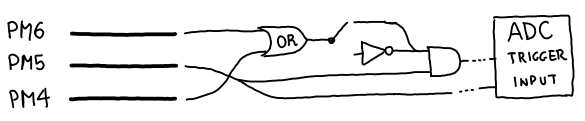
\includegraphics[width=8 cm]{anti_prov}
	\caption{schema dei collegamenti utilizzati rispettivamente per le misure in coincidenza ed anticoincidenza.}
	\label{anti_prov}
\end{figure}

\begin{figure}
	\hspace{-2cm}
	{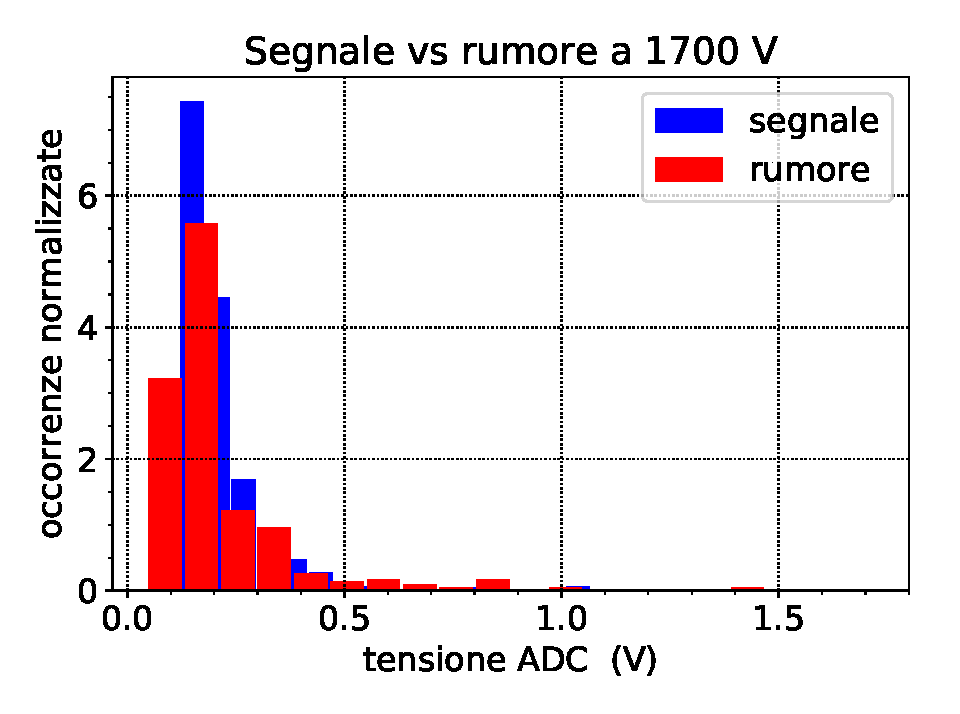
\includegraphics[width=8 cm]{1700}}
	\qquad
	{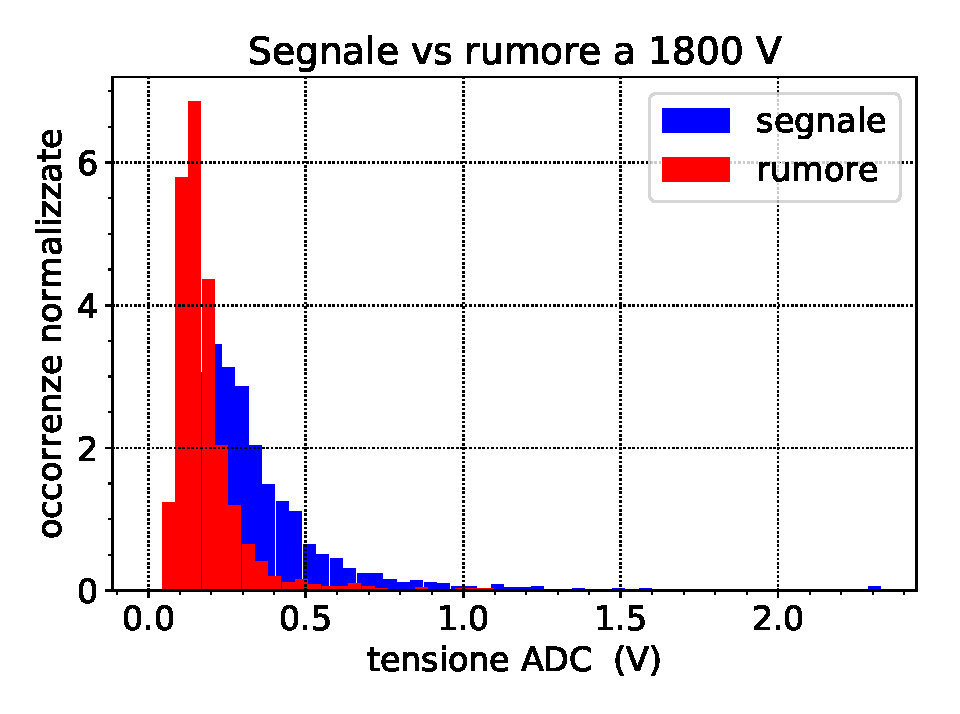
\includegraphics[width=8 cm]{1800}} 

	\hspace{-2cm}
	{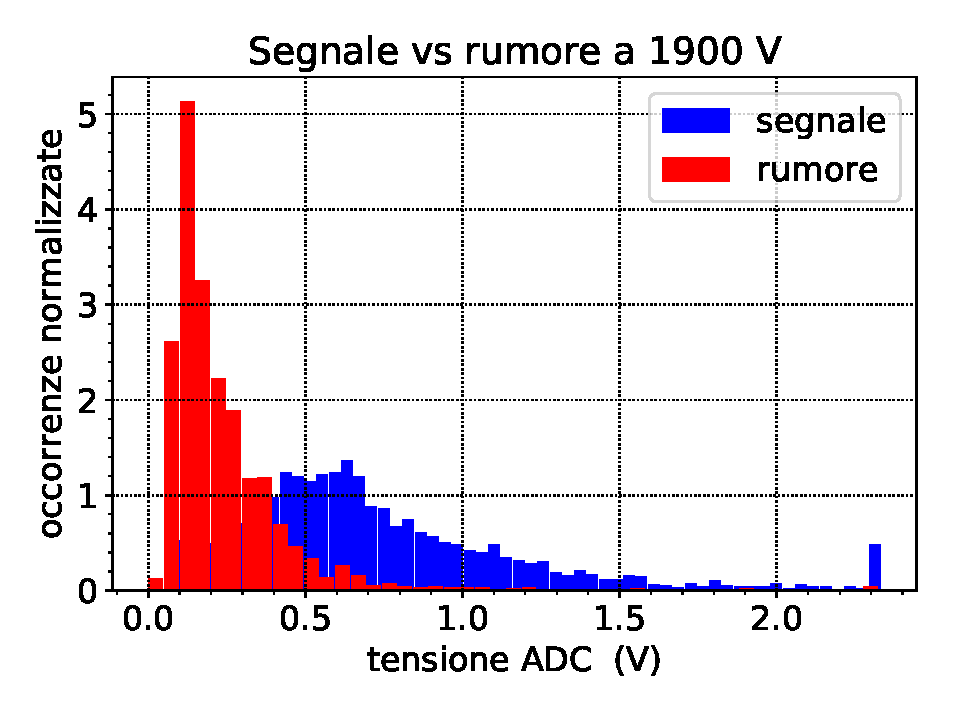
\includegraphics[width=8 cm]{1900}}
	\qquad
	{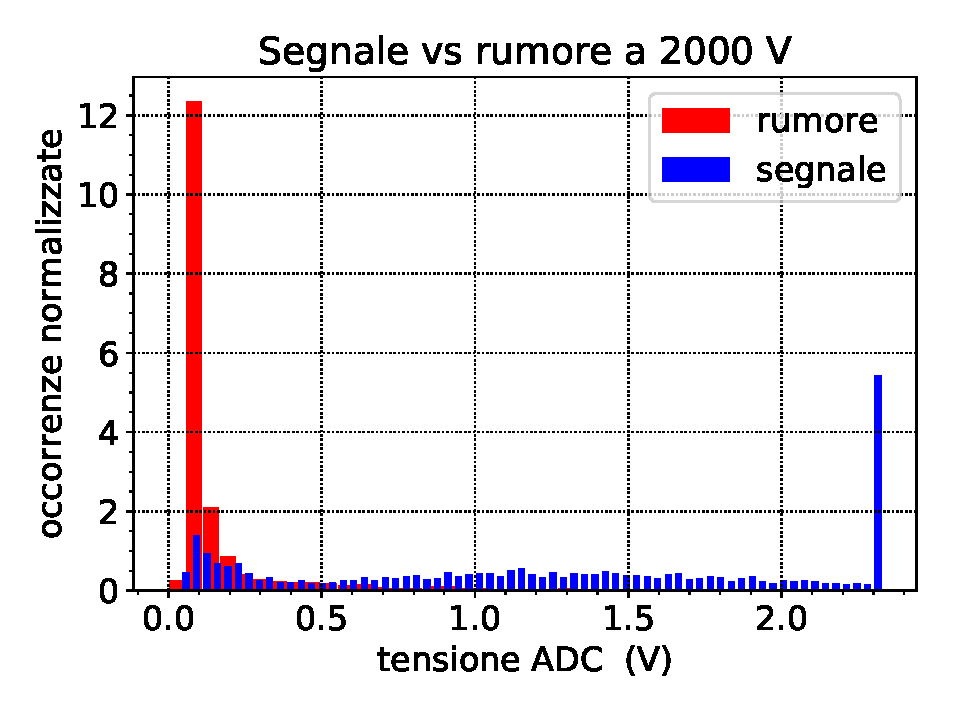
\includegraphics[width=8 cm]{2000}}
	\caption{Istogrammi che rappresentano il variare degli spettri di segnale e rumore per le tensioni più significative.
	A \SI{2000}V sulla sinistra si può notare un picco del segnale nella regione ad alto rumore.}
	\label{quattro}
\end{figure}

Analizziamo lo spettro in energia rilasciata del segnale e lo confrontiamo con quello del rumore.
Per fare questa misura usiamo le espressioni logiche mostrate in \autoref{anti_prov}
misurando il rilascio di energia sul PM5:
per selezionare il rumore usiamo l'espressione $\neg$(PM6 | PM4) \& PM5
in modo da avere la maggior esclusione angolare dei raggi%
\footnote{Non c'è nessun modo di escludere i raggi che passano a $\theta$ abbastanza grande.};
per selezionare il segnale usiamo l'espressione corrispondente a quella del rumore cioè (PM6 | PM4) \& PM5
per minimizzare ulteriori possibili differenze tra le misure
e per poter fare la misura senza cambiare circuito.

Abbiamo acquisito i dati in entrambe le configurazioni spazzando
l'alimentazione del PMT5 da \SI{1600}{V} a \SI{2000}{V} con un intervallo di \SI{50}{V}.
I PM4 e PM6 avevano soglie a \SI{200}{mV} e alimentazione a \SI{1900}V.
In \autoref{quattro} mostriamo un campione significativo delle misure.

Particolare attenzione merita il confronto tra segnale e rumore
per una tensione di alimentazione del PM5 di \SI{2000}{V} (vedi \autoref{quattro}):
segnale e rumore sono molto distinti, ma nell'istogramma del segnale si nota un picco nella regione ad elevato rumore.
Esso comprende circa il \SI{15}\% di tutti gli eventi
ed è di molto superiore al rate di coincidenze casuali attese che,
in tutte le misure, ammontano a meno dell'1\%.
